\section{Análisis exploratorio complementario}\label{ap:eda}

Este apéndice reúne las figuras verificadas de análisis exploratorio sobre el panel histórico de $17$ centrales (\texttt{base\_planta\_dia.csv}, $12\,756$ filas planta--día) que respaldan las decisiones de depuración, causalidad y modelado descritas en las Secciones~\ref{sec:modelo} y~\ref{sec:datos}: cobertura temporal heterogénea por planta, distribución de horas reportadas por XM y episodios anómalos, estacionalidad anual bimodal, estructura de autocorrelación temporal y espacial, y comportamiento de las variables meteorológicas.

\begin{figure}[!htbp]
\centering
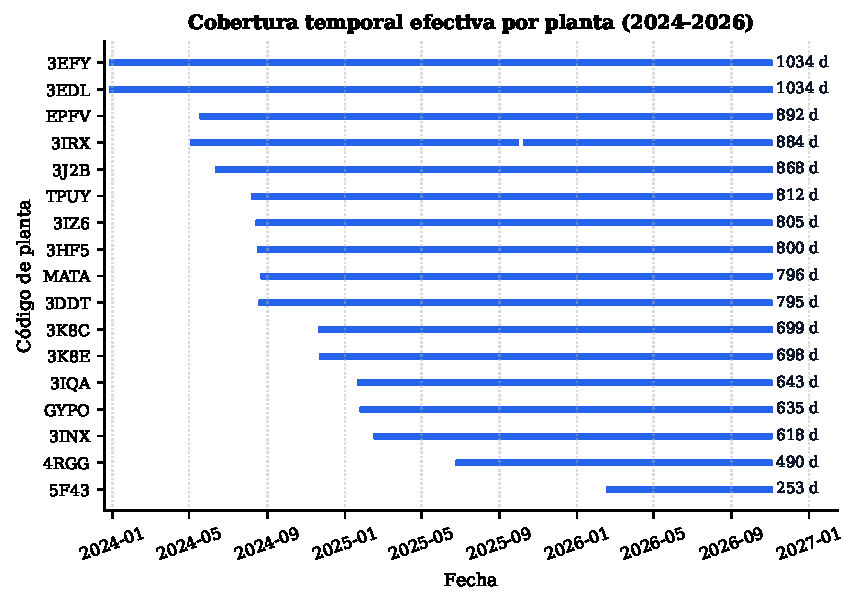
\includegraphics[width=0.92\textwidth]{figures/eda_cobertura_temporal.pdf}\\[0.5em]
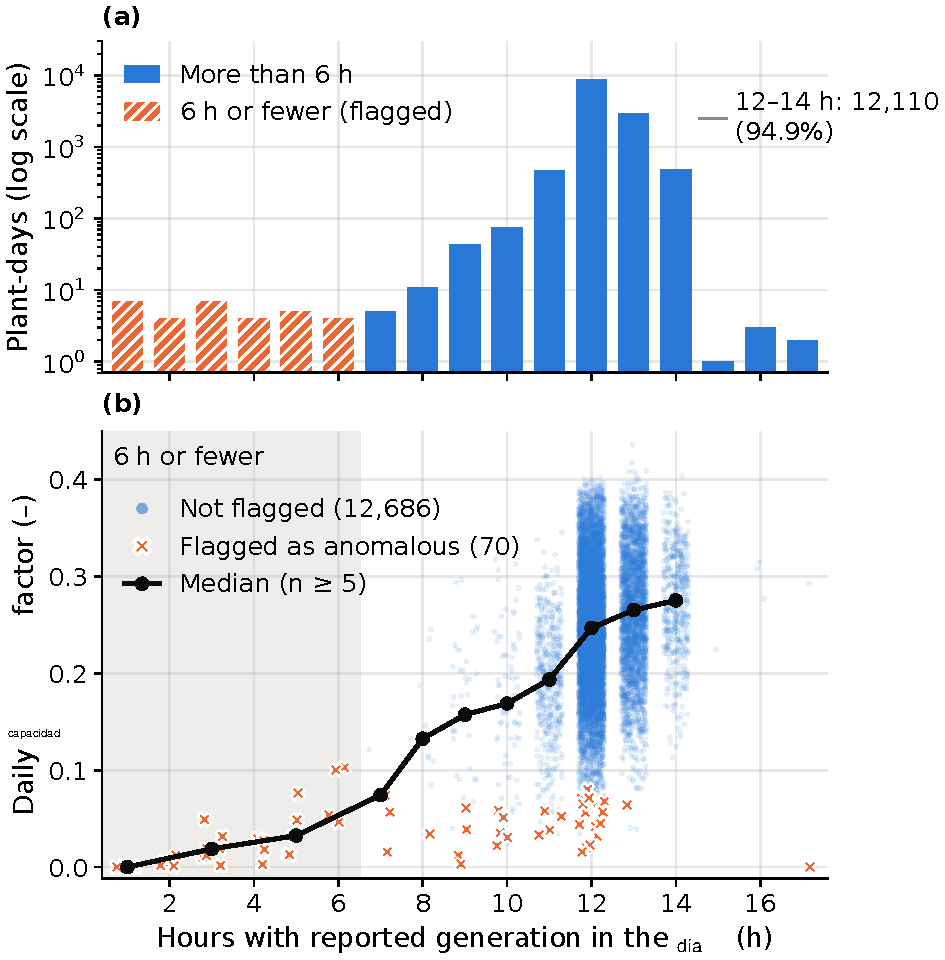
\includegraphics[width=0.92\textwidth]{figures/eda_horas_y_anomalos.pdf}
\caption{Cobertura temporal por planta ($251$ a $1\,032$ días útiles; arriba) y distribución de horas reportadas por XM junto con los días incompletos excluidos ($\le 6\text{ h}$; abajo).}
\label{fig:eda_cob_horas}
\end{figure}

\begin{figure}[!htbp]
\centering
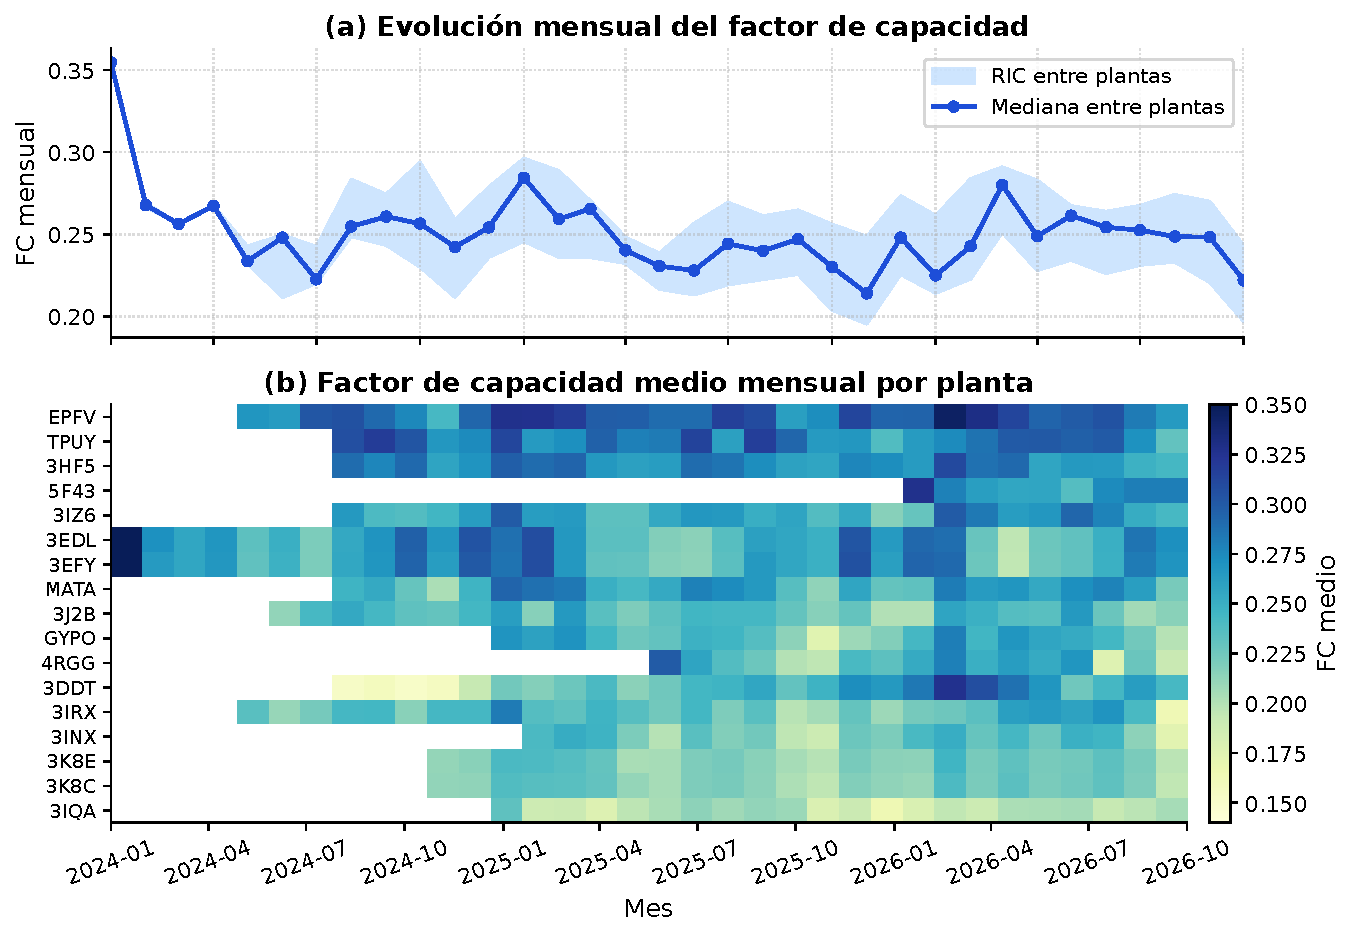
\includegraphics[width=0.92\textwidth]{figures/eda_estacionalidad.pdf}\\[0.5em]
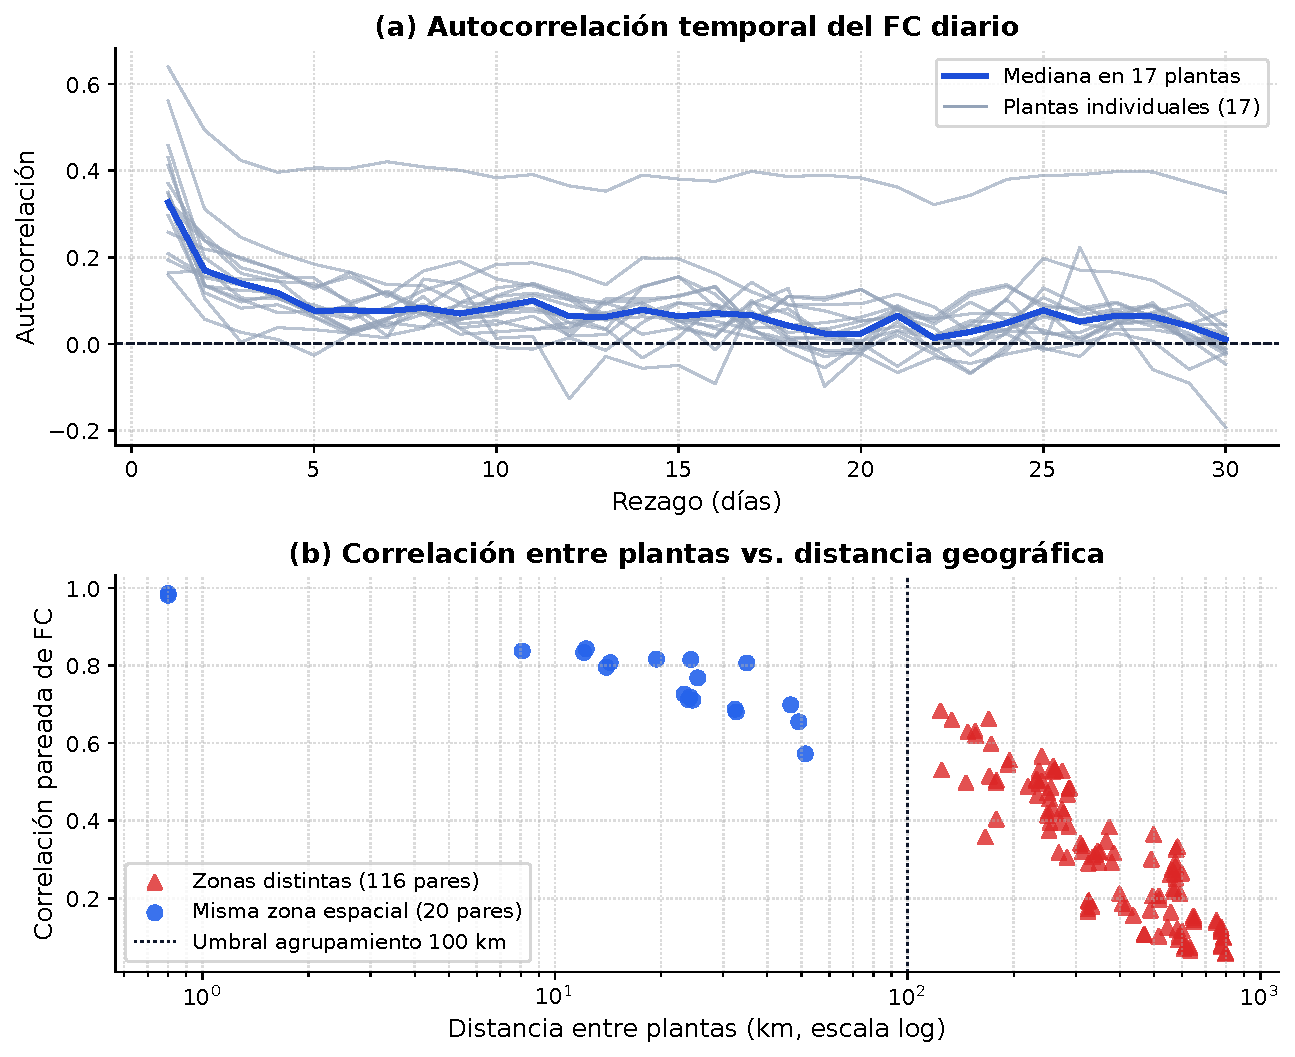
\includegraphics[width=0.92\textwidth]{figures/eda_dependencia.pdf}
\caption{Estacionalidad mensual del factor de capacidad (arriba) y estructura de autocorrelación temporal y correlación espacial entre centrales (abajo).}
\label{fig:eda_est_dep}
\end{figure}

\begin{figure}[!htbp]
\centering
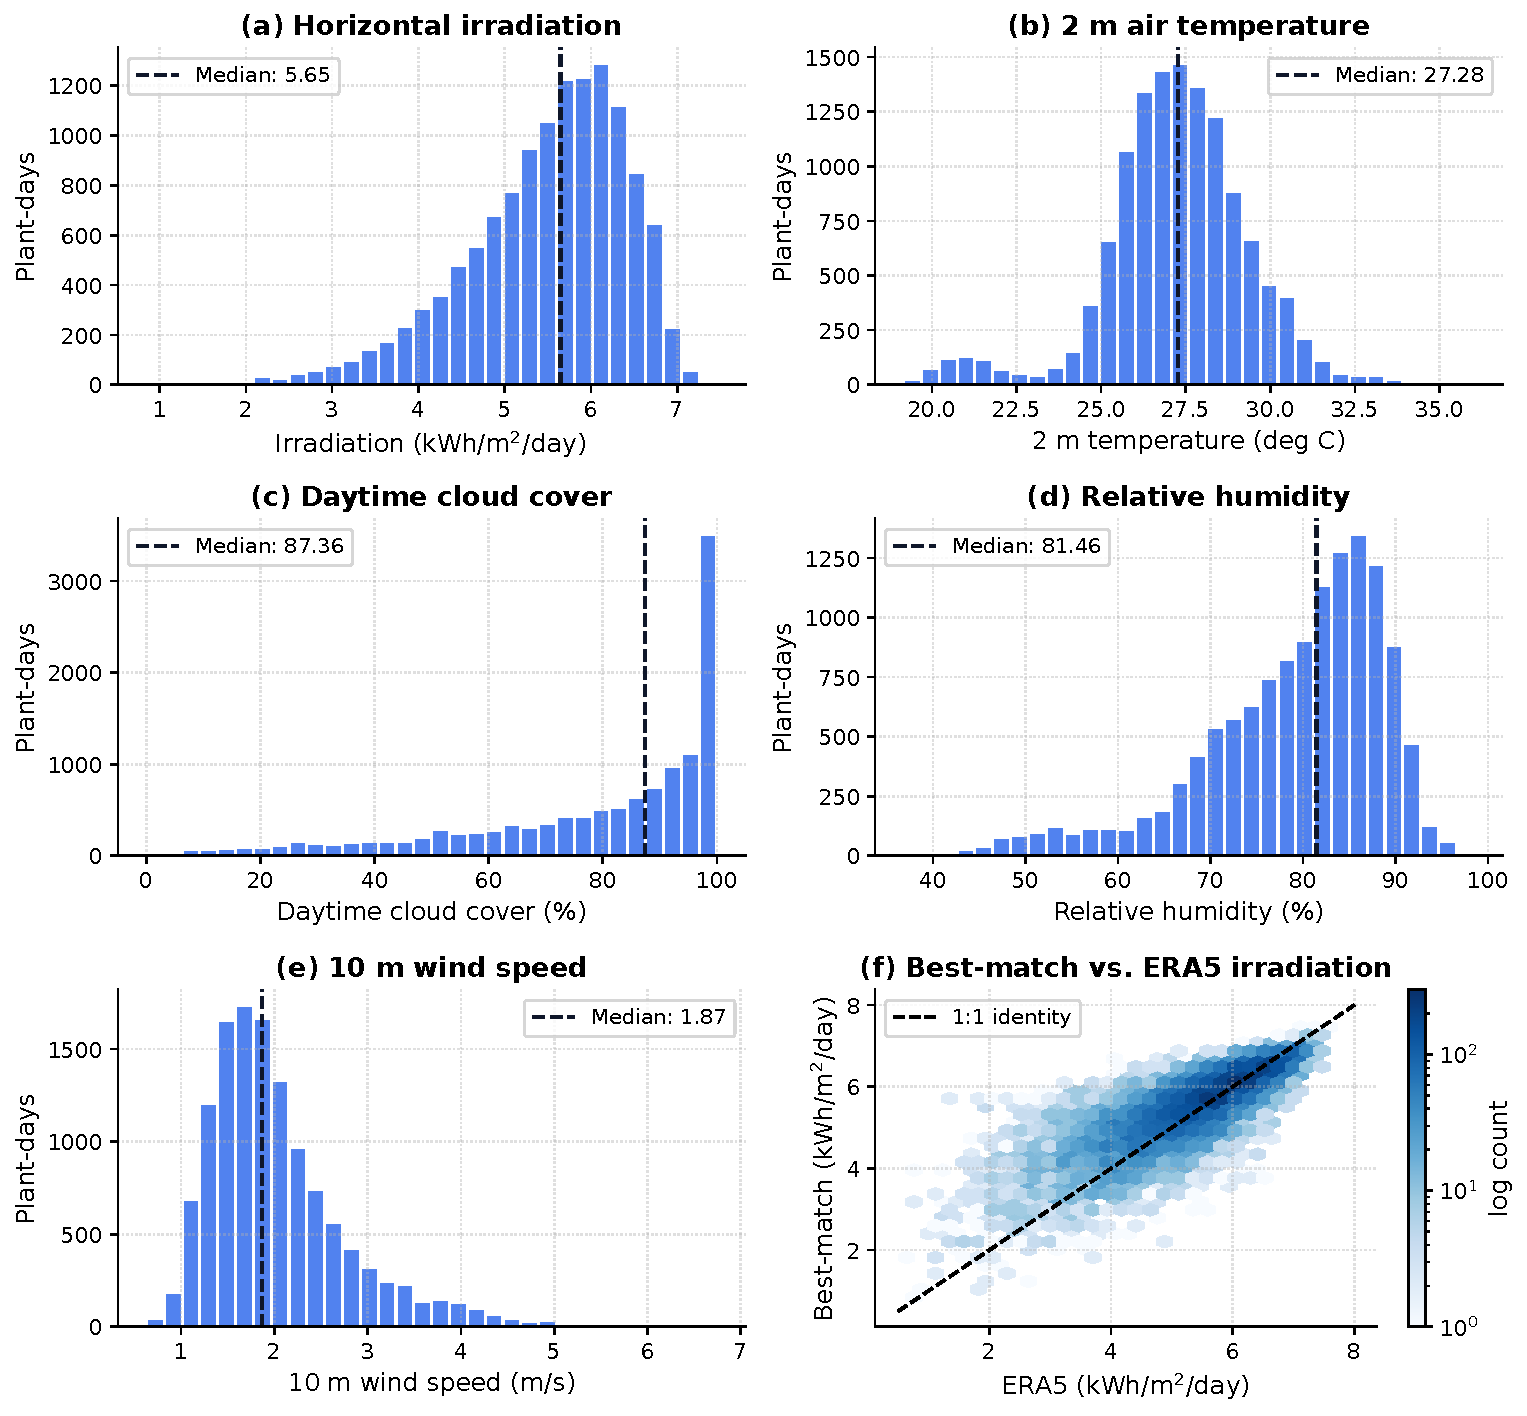
\includegraphics[width=0.92\textwidth]{figures/eda_clima.pdf}
\caption{Distribución y dinámica de las variables meteorológicas pronosticadas sobre la cohorte.}
\label{fig:eda_clima}
\end{figure}
